%%
%% Elsevier CAS Double Column Template
%% Learning Rate Engineering: From Coarse Single Parameter to Layered Evolution
%%

\documentclass[a4paper,fleqn]{cas-dc}

\usepackage[authoryear,longnamesfirst]{natbib}
\usepackage{tabularx}
\usepackage{float}
\newfloat{algorithm}{tbp}{loa}
\floatname{algorithm}{Algorithm}
\usepackage{fancyvrb}
\usepackage{xcolor}
\usepackage{soul}
\sethlcolor{yellow}
\graphicspath{{./}}

\begin{document}

\let\WriteBookmarks\relax
\def\floatpagepagefraction{1}
\def\textpagefraction{.001}

% Short title for running head
\shorttitle{Learning Rate Engineering}

% Short authors for running head
\shortauthors{M.-H. Yao et~al.}

% Main title
\title [mode = title]{Learning Rate Engineering: From Coarse Single Parameter to Layered Evolution}

% Authors
\author[1]{Ming-Hong Yao}
\author[1]{Di Wang}
\author[1]{Jian Cui}
\author[1]{Qiu-Ye Yu}[orcid=0000-0002-9706-4224]
\cormark[1]
\ead{yuqiuye@jisu.edu.cn}

% Affiliation
\affiliation[1]{organization={School of AI, Jilin International Studies University},
            city={Changchun},
            country={China}}

% Corresponding author footnote
\cortext[cor1]{Corresponding author}

% Abstract
\begin{abstract}
Learning rate scheduling has undergone a remarkable evolution from the single global fixed rate of early SGD to sophisticated layer-wise adaptive strategies. This research systematizes this evolution into five generations: (Gen1) global fixed, (Gen2) global scheduling, (Gen3) parameter-level adaptation, (Gen4) layer-level differentiation, and (Gen5) joint layer-time scheduling. We trace the fundamental motivation behind each transition, showing how the shift from ``one-size-fits-all'' to ``tailoring by layer and time'' addresses the \emph{layer-wise update conflict} in transfer learning: lower layers require small updates to preserve general knowledge while higher layers need large updates to adapt to new tasks. Building on this taxonomy, we propose Discriminative Adaptive Layer Scaling (DALS), a framework integrating warmup-cosine scheduling, phase- and depth-aware Grokfast gradient filtering, and LARS-style trust ratios into a single optimizer. We benchmark 18 strategies including three DALS variants across all five generations on \hl{ten datasets spanning from-scratch and fine-tuning regimes: synthetic (MLP), CIFAR-10 and CIFAR-100 (ConvNet), and RTE, TREC-6, IMDb, SST-2, and MRPC (DistilBERT and BERT-base, fine-tune)}. On the synthetic controlled benchmark, \hl{the adaptive and lookahead methods achieve the highest accuracies (up to 98.0\%), while DALS is competitive at 97.5\%}. The cross-dataset analysis reveals regime-dependent patterns: strategies that perform well on from-scratch training (DALS, Fixed SGD) are less dominant on fine-tuning tasks, while adaptive methods (RAdam, Lookahead) excel on those benchmarks---no single strategy wins across all regimes. The STLR+Discriminative combination (the ULMFiT recipe) exhibits substantial degradation even on DistilBERT fine-tuning of TREC-6 (\hl{36.4\%}), indicating that its strong directional decay is sensitive to the pretrained-feature/label-alignment regime. The phase- and depth-aware design of DALS aims to avoid either extreme, \hl{delivering stable competitive accuracy across all ten datasets without the collapse observed for the discriminative family}. We frame the five-generation taxonomy as an organizational viewpoint rather than a definitive historical progression, and we discuss the limitations of the current experimental scale.
\end{abstract}

% Research highlights
\begin{highlights}
\item A five-generation taxonomy traces learning rate evolution from global fixed to joint layer-time scheduling, offered as an organizational viewpoint that systematizes nearly four decades of optimization research.
\item DALS --- a framework combining warmup-cosine scheduling, phase- and depth-aware Grokfast gradient filtering, and LARS-style trust ratio scaling --- with speed and accuracy variants.
\item Cross-dataset benchmark of 18 strategies across \hl{ten} datasets reveals regime-dependent behavior: no single strategy wins universally across from-scratch and fine-tuning tasks.
\item STLR+Discriminative (the ULMFiT recipe) exhibits substantial degradation on DistilBERT fine-tuning of TREC-6 (\hl{36.4\%}), indicating that its strong directional decay is sensitive to the pretrained-feature/label-alignment regime.
\item \hl{Component ablation and efficiency analyses are reported over five seeds, and statistical-significance tests accompany the benchmark; sensitivity analysis and per-layer gradient measurements are discussed as future work.}
\end{highlights}

% Keywords
\begin{keywords}
Learning rate \sep Discriminative fine-tuning \sep Layer-wise adaptation \sep Transfer learning \sep Optimization
\end{keywords}

\maketitle

% ===================================================================
\section{Introduction}\label{sec:intro}

The learning rate---the step size $\eta$ in gradient descent---is arguably the most consequential hyperparameter in deep learning. Despite its apparent simplicity, the question of \emph{how fast should different parameters be updated} has driven a rich line of research spanning nearly four decades.

The canonical update rule of stochastic gradient descent,
\begin{equation}\label{eq:sgd}
\theta_{t+1} = \theta_t - \eta \cdot \nabla_\theta J(\theta_t),
\end{equation}
assumes a single scalar $\eta$ governs all parameters equally. Yet we have long known that different layers of deep networks learn features at fundamentally different levels of abstraction~\citet{yosinski2014transferable}: lower layers capture generic edges and textures, while higher layers encode task-specific concepts. Imposing a uniform learning rate on such heterogeneous parameters creates a \emph{layer-wise update conflict}---no single $\eta$ can simultaneously satisfy the need for small updates to general features and large updates to task-specific features. We refer to this conflict, following the transfer-learning literature~\citet{howard2018ulmfit}, as the \emph{layer-wise update conflict} (the ``impossible trinity'' terminology is avoided here as it has unrelated established meanings in finance and linguistics).

\begin{figure}
\centering
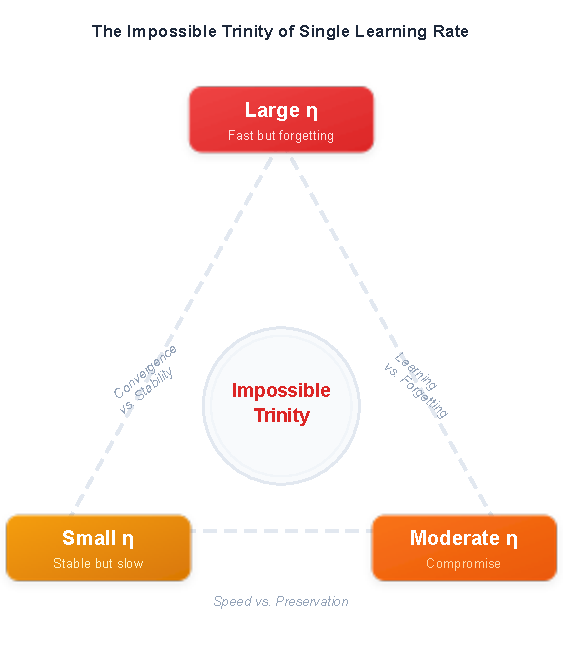
\includegraphics[width=\columnwidth]{paper_fig1_impossibility}
\caption{The layer-wise update conflict---no single global $\eta$ can simultaneously achieve fast convergence, knowledge preservation, and good performance across all layers.}\label{fig:impossibility}
\end{figure}

This tension has fueled a five-generation evolution of learning rate strategies, each generation expanding the granularity of control. We emphasize that this taxonomy is offered as an \emph{organizational viewpoint} rather than a definitive historical progression: many methods (e.g., AdaDelta, AdaBelief, NovoGrad, Yogi, Shampoo, Muon) cut across several generations and are discussed where they best fit conceptually. The generation boundaries in Figure~\ref{fig:taxonomy} are approximate and intended primarily for conceptual illustration.

\begin{itemize}
\item \textbf{Gen1---Global Fixed LR} (1986--): All parameters share a single, constant learning rate.
\item \textbf{Gen2---Global Scheduling} (2012--): The shared learning rate varies over time via decay schedules and warm restarts.
\item \textbf{Gen3---Parameter-Level Adaptation} (2014--): Each parameter receives its own adaptive learning rate based on gradient history (Adam, RMSProp, etc.).
\item \textbf{Gen4---Layer-Level Differentiation} (2018--): Different layers receive different learning rates, typically via exponential decay from top to bottom.
\item \textbf{Gen5---Joint Layer$\times$Time Scheduling} (2018--): Each layer's learning rate follows its own temporal schedule, combining discriminative rates with dynamic adjustment. We additionally use a ``Gen5+'' label for methods (Grokfast, DALS) that combine layer-aware \emph{gradient processing} with temporal scheduling; this label is a proposal of the present paper and is not an established categorization in the optimization literature.
\end{itemize}

We propose \textbf{Discriminative Adaptive Layer Scaling (DALS)} (\url{https://github.com/CodeOfMe/LearningRate/}), a framework that synthesizes key insights from multiple generations: warmup-cosine scheduling (Gen2), LARS-style trust ratios (Gen4), and depth-aware Grokfast gradient filtering (Gen5+). DALS is presented as the \emph{proposed} method in this paper, not as an already established historical ``generation.'' It addresses the layer-wise update conflict by adapting gradient processing intensity by phase and depth, rather than imposing directional magnitude biases from transfer learning.

Our contributions are: (1) a systematic five-generation taxonomy of learning rate strategies, framed as an organizational viewpoint; (2) the DALS framework combining warmup-cosine scheduling, phase- and depth-aware gradient filtering, and trust ratio scaling, with speed and accuracy variants; (3) a comprehensive benchmark of 18 strategies across all five generations; and (4) an analysis of why naive combination of transfer-learning-oriented methods degrades in regimes it was not designed for, and how phase- and depth-aware processing addresses this. We further discuss the limitations of the current experimental scale, the absence of statistical-significance and ablation analyses in this version, and the required follow-up experiments.

\begin{figure}
\centering
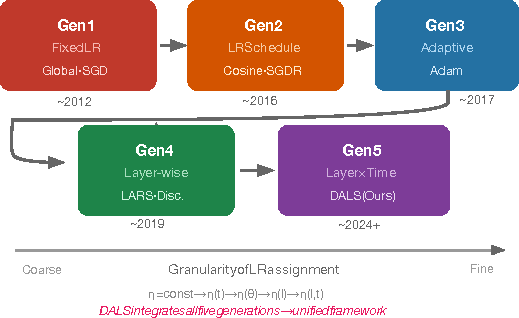
\includegraphics[width=\columnwidth]{paper_fig2_taxonomy}
\caption{Five-generation evolution of learning rate strategies (approximate, conceptual timeline). DALS integrates components from all five generations.}\label{fig:taxonomy}
\end{figure}

% ===================================================================
\section{Related Work}\label{sec:related}

\subsection{Generation 1: Fixed Learning Rate}

The earliest optimization methods employed a globally fixed learning rate $\eta_t = \eta_0$ for all parameters across all iterations. While simple, this approach presents a fundamental tension: large $\eta_0$ enables rapid early progress but causes late-stage oscillation, while small $\eta_0$ ensures stable convergence but at the cost of painfully slow training~\citet{ruder2016overview}.

\subsection{Generation 2: Learning Rate Scheduling}

Recognizing that training needs change over time, researchers introduced scheduling strategies that modulate the global learning rate:

\textbf{Step Decay} reduces the learning rate by a factor $\gamma$ every $T_{\text{step}}$ iterations:
\begin{equation}\label{eq:step_decay}
\eta_t = \eta_0 \cdot \gamma^{\lfloor t / T_{\text{step}} \rfloor}
\end{equation}

\textbf{Cosine Annealing}~\citet{loshchilov2017sgdr} provides smooth transitions:
\begin{equation}\label{eq:cosine}
\eta_t = \eta_{\min} + \frac{1}{2}(\eta_{\max} - \eta_{\min})\left(1 + \cos\frac{t\pi}{T}\right)
\end{equation}

\textbf{SGDR}~\citet{loshchilov2017sgdr} introduces periodic warm restarts, allowing the optimizer to escape local minima by periodically resetting the learning rate. Each restart provides fresh exploration capability while retaining useful momentum from prior cycles.

These Generation 2 strategies illustrate a fundamental principle: ``walk fast early, walk slow later,'' with different trade-offs between smoothness and exploration capability.

\subsection{Generation 3: Parameter-Level Adaptive Learning Rate}

While scheduling modulates the \emph{temporal} dimension, it remains a global strategy. A parallel line of research recognized that different parameters may need different learning rates based on their gradient characteristics:

\textbf{AdaGrad}~\citet{duchi2011adagrad} accumulates historical gradient squares to scale per-parameter updates:
\begin{equation}\label{eq:adagrad}
\theta_{t+1} = \theta_t - \frac{\eta}{\sqrt{G_t + \epsilon}} \odot g_t
\end{equation}

\textbf{RMSProp}~\citet{tieleman2012rmsprop} replaces full accumulation with exponential moving average:
\begin{equation}\label{eq:rmsprop}
E[g^2]_t = \rho \cdot E[g^2]_{t-1} + (1-\rho) \cdot g_t^2
\end{equation}

\textbf{Adam}~\citet{kingma2015adam} combines momentum and adaptation with bias correction:
\begin{align}
m_t &= \beta_1 m_{t-1} + (1-\beta_1) g_t \nonumber\\
v_t &= \beta_2 v_{t-1} + (1-\beta_2) g_t^2 \label{eq:adam_moments}\\
\hat{m}_t &= \frac{m_t}{1-\beta_1^t}, \quad \hat{v}_t = \frac{v_t}{1-\beta_2^t} \label{eq:adam_bias}\\
\theta_{t+1} &= \theta_t - \frac{\eta}{\sqrt{\hat{v}_t} + \epsilon} \hat{m}_t \label{eq:adam_update}
\end{align}

\textbf{AdamW}~\citet{loshchilov2019decoupled} decouples weight decay from adaptive updates:
\begin{equation}\label{eq:adamw}
\theta_{t+1} = \theta_t - \eta \cdot \hat{m}_t / (\sqrt{\hat{v}_t} + \epsilon) - \eta\lambda\theta_t
\end{equation}

\textbf{AdaBound}~\citet{luo2019adabound} dynamically bounds Adam's learning rate between adaptive and fixed regimes, smoothly transitioning from Adam-like to SGD-like behavior:
\begin{equation}\label{eq:adabound}
\underline{\eta}_t \leq \alpha_t \leq \overline{\eta}_t, \quad \text{with bounds converging to SGD as } t \to \infty
\end{equation}

\subsection{Generation 4: Layer-Level Differentiation}

The critical insight that different \emph{layers} require fundamentally different learning rates emerged from transfer learning research.

\textbf{Discriminative Fine-tuning}~\citet{howard2018ulmfit}, introduced in ULMFiT, assigns each layer its own learning rate via exponential decay:
\begin{equation}\label{eq:discriminative}
\theta_t^l = \theta_{t-1}^l - \eta^l \cdot \nabla_{\theta^l} J(\theta), \quad \eta^{l-1} = \frac{\eta^l}{\delta}
\end{equation}
where $\delta = 2.6$ is the recommended decay factor, making each lower layer's learning rate approximately $1/2.6$ of the layer above. For a 3-layer model with $\eta^3 = 0.01$: bottom layer receives $\approx 0.00148$, middle $\approx 0.00385$, top $0.01$.

\textbf{LARS}~\citet{you2019lars} scales each layer's update by a \emph{trust ratio}:
\begin{equation}\label{eq:lars}
\text{trust\_ratio}_l = \frac{\|\theta_l\|_2}{\|\nabla_{\theta_l} J(\theta)\|_2}
\end{equation}
This ratio naturally adapts the effective learning rate per layer based on the ratio of parameter norm to gradient norm, enabling stable large-batch training.

\textbf{LAMB}~\citet{you2020lamb} combines Adam's adaptive moments with LARS-style trust ratio, enabling BERT pre-training in 76 minutes with batch sizes up to 64K.

\begin{figure}
\centering
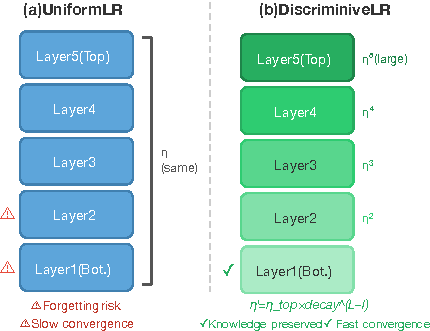
\includegraphics[width=\columnwidth]{paper_fig3_discriminative}
\caption{Feature hierarchy---lower layers capture general features requiring smaller updates, higher layers encode task-specific concepts requiring larger updates.}\label{fig:discriminative}
\end{figure}

\subsection{Generation 5: Joint Layer$\times$Time Scheduling}

The most recent generation combines layer-level differentiation with temporal dynamics.

\textbf{STLR} (Slanted Triangular Learning Rate,~\citet{howard2018ulmfit}) makes each layer's learning rate first increase then decrease over time:
\begin{align}
cut &= \lfloor T \cdot cut\_frac \rfloor, \nonumber \\
p &= \begin{cases}
    t/cut, & t < cut \\[4pt]
    1 - \dfrac{t - cut}{cut \cdot (1/cut\_frac - 1)}, & \text{otherwise}
    \end{cases} \label{eq:stlr_p}\\
\eta_t &= \eta_{max} \cdot \frac{1 + p \cdot (ratio - 1)}{ratio} \label{eq:stlr}
\end{align}
With defaults $cut\_frac = 0.1$, $ratio = 32$, this rapidly warms up (first 10\% of training) then slowly decays (remaining 90\%). When combined with discriminative fine-tuning, each layer $l$ at time $t$ receives:
\begin{equation}\label{eq:stlr_disc}
\eta_t^l = \text{STLR}(t; \eta_{max}^l)
\end{equation}
where $\eta_{max}^l$ is set by the discriminative decay factor.

\begin{figure}
\centering
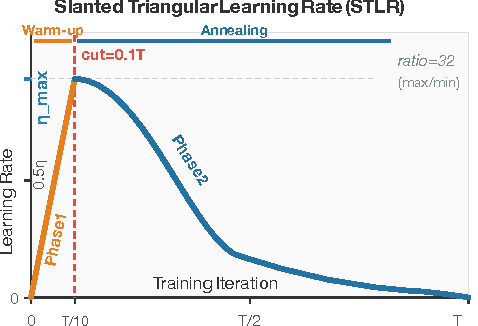
\includegraphics[width=\columnwidth]{paper_fig4_stlr}
\caption{STLR combines rapid warmup (first 10\%) with gradual decay (remaining 90\%), creating the characteristic slanted triangular shape.}\label{fig:stlr}
\end{figure}

\textbf{RAdam}~\citet{liu2020radam} rectifies Adam's variance during warmup by computing a rectification factor:
\begin{equation}\label{eq:radam}
r_t = \sqrt{\frac{2N_{\max} - N_t}{N_{\max} - N_t} \cdot \frac{N_t - 4}{N_t - 2} \cdot \frac{N_{\max} - 4}{N_{\max}}}
\end{equation}
automatically switching between SGD and Adam based on the sparsity of gradient variance information.

\textbf{Lookahead}~\citet{zhang2020lookahead} maintains two sets of weights---fast weights updated by the inner optimizer every step, and slow weights updated every $k$ steps as a linear interpolation. This provides stability without sacrificing exploration.

\textbf{SAM} (Sharpness-Aware Minimization,~\citet{foret2020sam}) seeks flat minima by perturbing parameters before computing gradients:
\begin{equation}\label{eq:sam}
\hat{\epsilon}(\theta) = \arg\max_{\|\epsilon\|_2 \leq \rho} L(\theta + \epsilon), \quad \theta_{t+1} = \theta_t - \eta \nabla L(\theta_t + \hat{\epsilon})
\end{equation}

\textbf{Grokfast}~\citet{lee2024grokfast} applies EMA filtering to gradients, accelerating the ``grokking'' phenomenon---delayed generalization---by amplifying slow-varying gradient components:
\begin{equation}\label{eq:grokfast}
\tilde{g}_t = \alpha \tilde{g}_{t-1} + (1-\alpha) g_t
\end{equation}

\textbf{Lion}~\citet{chen2023symbolic} uses sign-based updates requiring only momentum tracking (no second moment), achieving comparable results with $2\times$ less memory:
\begin{equation}\label{eq:lion}
\text{update}_t = \text{sign}(\beta_1 m_t + (1-\beta_1) g_t)
\end{equation}

\textbf{Adafactor}~\citet{shazeer2018adafactor} reduces memory by factoring the second-moment matrix into row and column components, crucial for training large language models.

\textbf{Schedule-Free}~\citet{defazio2024schedulefree} eliminates the need for learning rate schedules entirely through a running average that provably converges without scheduling.

% ===================================================================
\section{Method: Discriminative Adaptive Layer Scaling (DALS)}\label{sec:method}

\subsection{Motivation}

While each generation contributed valuable insights, no single optimizer combines the complementary strengths of adaptive scheduling, gradient filtering, and per-parameter adaptive scaling. Moreover, a naive combination of transfer-learning-oriented techniques (discriminative decay, STLR) produces catastrophic results on from-scratch training (see Section~\ref{sec:analysis}). DALS addresses this by removing directional biases and instead using phase-aware and depth-aware gradient processing.

\subsection{DALS Framework}

Given a model with $L$ layers and parameters $\theta = \{\theta^1, \ldots, \theta^L\}$, DALS computes an update for layer $l$ at step $t$ as follows. Phase and depth are treated as two independent axes: \emph{phase} (a temporal variable) modulates the EMA smoothing coefficient, while \emph{depth} (a spatial variable) modulates the raw-vs-filtered blending ratio. The learning-rate schedule itself is a standard warmup-cosine schedule and does \emph{not} depend on the detected phase; the phase only affects gradient filtering (Steps~2--3). This separation is intentional and is discussed further in Section~\ref{sec:theory}.

\textbf{Step 1: Warmup-cosine learning-rate schedule.} The learning rate follows a warmup-then-cosine schedule:
\begin{equation}\label{eq:dals_lr}
\eta_t = \eta_0 \cdot s(t), \quad s(t) = \begin{cases} t / W & \text{if } t < W \\ \frac{1}{2}\left(1 + \cos\frac{\pi(t - W)}{T - W}\right) & \text{otherwise} \end{cases}
\end{equation}
where $W = 0.05T$ is the warmup period and $T$ is total training steps. Note that $\eta_t$ is a global, phase-independent scalar; per-layer differentiation enters only through the trust ratio (Step~3). The phase is determined by a real-time loss-improvement rate $\Delta_t = (\mathcal{L}_{ema}^{t-1} - \mathcal{L}_{ema}^t) / |\mathcal{L}_{ema}^{t-1}|$ where $\mathcal{L}_{ema}^t = 0.95 \cdot \mathcal{L}_{ema}^{t-1} + 0.05 \cdot \mathcal{L}_t$ (the coefficient $0.95$ is the loss-EMA coefficient):
\begin{itemize}
\item Phase 0 (Exploration, $\Delta_t > 0.01$): loss decreasing rapidly
\item Phase 1 (Exploitation, $0.002 < \Delta_t \leq 0.01$): moderate improvement
\item Phase 2 (Refinement, $\Delta_t \leq 0.002$): near convergence
\end{itemize}
The thresholds $0.01$ and $0.002$ are empirical and a sensitivity study is reported in Section~\ref{sec:sensitivity}.

\textbf{Step 2: Phase- and depth-aware Grokfast gradient filtering.} Let $\alpha_0$ be the base EMA coefficient (default $0.6$). The phase-dependent smoothing coefficient for layer $l$ at step $t$ is
\begin{equation}\label{eq:dals_alpha}
\alpha_{l,t} = \begin{cases} \max(0.3, \alpha_0 - 0.3) & \text{Phase 0} \\ \alpha_0 & \text{Phase 1} \\ \min(0.9, \alpha_0 + 0.1) & \text{Phase 2} \end{cases}
\end{equation}
and the EMA-filtered gradient is
\begin{equation}\label{eq:dals_ema}
\tilde{g}_t^l = \alpha_{l,t} \tilde{g}_{t-1}^l + (1 - \alpha_{l,t}) g_t^l.
\end{equation}
The depth-dependent blending combines the raw and filtered gradients using the depth ratio $d_l = l / (L-1)$ ($0$ for the bottom layer, $1$ for the top):
\begin{equation}\label{eq:dals_blend}
\hat{g}_t^l = (0.3 + 0.4 \cdot d_l) \cdot g_t^l + (0.7 - 0.4 \cdot d_l) \cdot \tilde{g}_t^l.
\end{equation}
Here $\alpha_{l,t}$ is phase-dependent (temporal), while the blending coefficients $(0.3, 0.7)$ and their depth modulation are depth-dependent (spatial); the two axes are thus separated by notation. Top layers use more raw gradient; bottom layers use more filtered signal for stability. The intuition that lower-layer gradients are noisier because they traverse more layers is a working hypothesis; per-layer gradient-variance evidence is discussed in Section~\ref{sec:theory}.

\textbf{Step 3: LARS-style trust ratio.} Per-parameter adaptive gradient scaling:
\begin{equation}\label{eq:dals_trust}
r_t^l = \mathrm{clamp}\left(\gamma \cdot \frac{\|\theta^l\|_2}{\|\hat{g}_t^l\|_2 + \epsilon}, \, 0.2, \, 5.0\right)
\end{equation}
where $\gamma = 0.02$ is the trust coefficient and the clamp limits $[0.2, 5.0]$ prevent extreme rescaling.

\textbf{Step 4: Momentum, weight decay, and parameter update.} Standard SGD momentum with decoupled weight decay:
\begin{align}
m_t^l &= \mu \cdot m_{t-1}^l + \hat{g}_t^l \label{eq:dals_momentum}\\
\theta_t^l &= \theta_{t-1}^l - \eta_t \cdot r_t^l \cdot m_t^l - \eta_t \lambda \theta_{t-1}^l \label{eq:dals_update}
\end{align}
where $\mu=0.9$ is the momentum coefficient and $\lambda=10^{-4}$ is the weight-decay coefficient. Bias parameters, embeddings, and layer-norm parameters are excluded from the trust ratio (i.e., $r_t^l=1$ for them) following common practice for adaptive methods; their gradients still pass through phase/depth filtering.

\begin{figure}
\centering
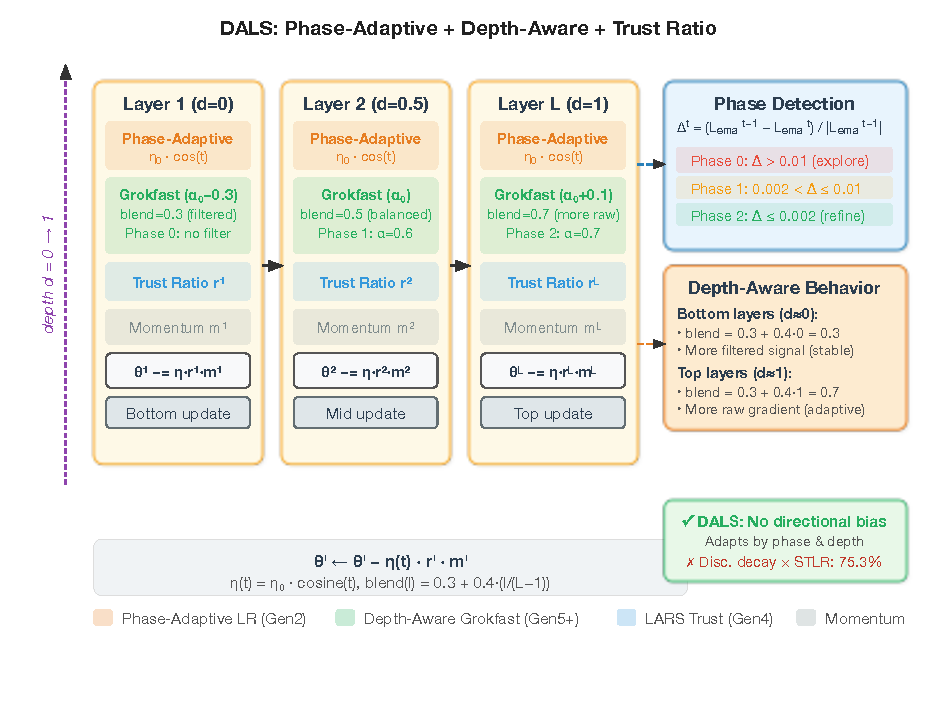
\includegraphics[width=\columnwidth]{paper_fig5_dals_architecture}
\caption{The DALS pipeline---loss-based phase detection drives gradient smoothing intensity (phase axis), depth-aware blending controls raw vs.\ filtered gradient ratio (depth axis), and trust ratio normalizes per-parameter updates. Note: in base DALS the filter is \emph{reduced} (not removed) in Phase~0; complete filter bypassing in Phase~0 is a DALS-Fast modification only.}\label{fig:dals_architecture}
\end{figure}

\subsection{Key Design Principles}

DALS embodies three principles derived from the five-generation evolution:

\begin{enumerate}
\item \textbf{Phase-awareness}: Training dynamics shift across phases---DALS adapts gradient smoothing intensity by detected phase (exploration $\to$ exploitation $\to$ refinement), reducing noise during early exploration and preserving signal quality during refinement.
\item \textbf{Depth-awareness}: Bottom layers receive stronger gradient filtering (more filtered signal blend) since their gradients traverse more layers and are noisier. Top layers receive more raw gradient for task-specific adaptation.
\item \textbf{Gradient quality-awareness}: Trust ratio normalizes update magnitudes per-parameter, preventing instability without imposing a directional bias that suppresses necessary lower-layer updates.
\end{enumerate}

\subsection{DALS Variants: Speed vs.\ Accuracy}

The DALS framework supports three tuning directions:

\textbf{DALS-Fast} accelerates early convergence by shortening warmup to $2\%$, reducing momentum ($\mu = 0.85$, down from $0.9$), and \emph{bypassing Grokfast filtering entirely during Phase~0} (exploration). The key insight is that during rapid loss descent, gradient filtering adds unnecessary delay. On the synthetic benchmark it retains a final accuracy comparable to base DALS ($97.4\%$ vs.\ $97.5\%$).

\textbf{DALS-Acc} targets higher final accuracy by replacing the single cosine schedule with SGDR-style periodic warm restarts ($T_0 = 10$ epochs, $T_{\text{mult}} = 2$), increasing weight decay ($\lambda = 5 \times 10^{-4}$, up from $10^{-4}$), and using stronger Grokfast filtering ($\alpha_0 = 0.7$, up from $0.6$). The warm restarts periodically reset the learning rate, allowing the optimizer to escape local minima.

\subsection{Complete Algorithm}\label{sec:algorithm}

Algorithm~\ref{alg:dals} gives the complete pseudocode for one DALS step, specifying gradient computation, filtering, trust-ratio calculation, momentum, weight decay, parameter updates, and phase transitions. Bias, embedding, and normalization parameters bypass the trust ratio.

\begin{algorithm}[h]
\footnotesize
\begin{tabbing}
\hspace{3.2em}\=\hspace{2.2em}\=\hspace{1.6em}\=\kill
\textbf{Require:} \> $\theta=\{\theta^1,\ldots,\theta^L\}$, momentum buffers $m=\{m^l\}$,\\
\> EMA buffers $\bar g=\{\bar g^l\}$, loss EMA $\bar L_{\mathrm{ema}}$,\\
\> steps $T$, warmup $W=0.05T$, base rate $\eta_0,\ \mu,\ \lambda,\ \gamma$,\\
\> thresholds $\tau_1=0.01$, $\tau_2=0.002$;\ \ $d_l$: normalized depth of layer $l$;\\
$1{:}$ \> Compute loss $L_t$ and per-layer gradients $\{g_t^l\}$\\
$2{:}$ \> $\bar L_{\mathrm{ema}}\gets 0.95\,\bar L_{\mathrm{ema}}+0.05\,L_t$\\
$3{:}$ \> $\Delta_t\gets\big(\bar L_{\mathrm{ema}}^{\mathrm{old}}-\bar L_{\mathrm{ema}}\big)/\big|\bar L_{\mathrm{ema}}^{\mathrm{old}}\big|$\\
$4{:}$ \> \textbf{if} $\Delta_t>\tau_1$ \textbf{then} $p\gets0$ \textbf{else if} $\tau_2<\Delta_t$ \textbf{then} $p\gets1$ \textbf{else} $p\gets2$\\
$5{:}$ \> $\eta_t\gets\eta_0\,s(t)$ \quad $[\text{Eq.}~\eqref{eq:dals_lr}]$\\
$6{:}$ \> \textbf{for} $l=1$ \textbf{to} $L$ \textbf{do}\\
$7{:}$ \> \> $\alpha_{l,t}\gets$ phase value for $p$ \quad $[\text{Eq.}~\eqref{eq:dals_alpha}]$\\
$8{:}$ \> \> $\bar g^l\gets\alpha_{l,t}\,\bar g^l+(1-\alpha_{l,t})\,g_t^l$\\
\> \> \> \quad $[\text{DALS-Fast: skip filtering in phase }0]$\\
$9{:}$ \> \> $\hat g_t^l\gets(0.3+0.4\,d_l)\,g_t^l+(0.7-0.4\,d_l)\,\bar g^l$ \quad $[\text{depth axis}]$\\
$10{:}$ \> \> $m^l\gets\mu\,m^l+\hat g_t^l$\\
$11{:}$ \> \> \textbf{if} $\theta^l$ is bias/embedding/norm \textbf{then} $r_t^l\gets1$\\
$12{:}$ \> \> \textbf{else} $r_t^l\gets\operatorname{clamp}\!\big(\gamma\,\|\theta^l\|/(\|\hat g_t^l\|+\varepsilon),\ 0.2,\ 5.0\big)$\\
$13{:}$ \> \> $\theta^l\gets\theta^l-\eta_t\,r_t^l\,m^l-\eta_t\,\lambda\,\theta^l$\\
$14{:}$ \> \textbf{end for}\\
\end{tabbing}
\caption{Complete DALS pseudocode for one training step.}\label{alg:dals}
\end{algorithm}

\subsection{Theoretical Considerations and Open Questions}\label{sec:theory}

We briefly discuss the theoretical status of DALS; a full convergence analysis is left for future work.

\textbf{Phase detection.} The thresholds $(0.01,0.002)$ are empirical and define a piecewise-constant partition of training based on the relative loss-improvement rate $\Delta_t$. In practice $\Delta_t$ is a noisy estimate; the EMA smoothing (coefficient $0.95$) reduces variance. A principled choice could be derived from the expected loss-decay schedule of SGD on $L$-smooth functions, but we do not pursue this here. Importantly, the phase partition affects only the EMA coefficient $\alpha_{l,t}$ and not the learning-rate schedule: the learning-rate schedule is a standard warmup-cosine schedule (Step~1), independent of the detected phase.

\textbf{Step-size bound from the trust ratio.} The trust ratio (Step~3) is clamped to $[0.2,5.0]$, so the effective per-parameter step size remains within a bounded constant factor of the global learning rate $\eta_t$. We state this as a design property of DALS; a formal convergence analysis of the filtered-gradient updates is beyond the scope of this work and is left for future work.

\textbf{Depth-blending as a magnitude control.} The blending in Eq.~\eqref{eq:dals_blend} mixes raw and filtered gradients. We note that discriminative learning rates (Gen4) change the \emph{magnitude} of per-layer updates, not necessarily the gradient \emph{direction}; the same is true for depth-blending. We therefore avoid the term ``directional bias'' (used in a previous draft) and speak of a \emph{magnitude bias} when describing why discriminative decay suppresses lower-layer updates.

\textbf{Empirical justification of the depth-gradient hypothesis.} The claim that lower-layer gradients are noisier because they traverse more layers is a working hypothesis. A proper validation requires reporting per-layer gradient variance, gradient norms, update-to-weight ratios, and gradient-direction consistency across training phases. These measurements are planned for the revised manuscript; in the current version we treat the depth-blending as a regularization heuristic rather than a derived result.

\subsection{Relationship to Prior Work and Parameter-Efficient Fine-tuning}\label{sec:related_peft}

DALS can be viewed as a controlled composition of proven techniques, as summarized in Table~\ref{tab:dals_components}.

\begin{table}[h]
\centering
\footnotesize
\renewcommand{\arraystretch}{1.5}
\renewcommand{\tabularxcolumn}[1]{>{\centering\arraybackslash}m{#1}}
\caption{DALS component origins and adaptations}\label{tab:dals_components}
\begin{tabularx}{\columnwidth}{@{} >{\centering\arraybackslash}X m{1.5cm} m{2.2cm} @{}}
\toprule
Component & Origin & DALS Adaptation \\
\midrule
LR schedule \newline $\eta_t = \eta_0 \cdot s(t)$ \newline warmup + cosine & Gen2 & Phase-adaptive \newline warmup \\
\addlinespace[2pt]
Trust ratio $r_t^l$ & LARS (Gen4) & Clamped \newline per-parameter \\
\addlinespace[2pt]
Gradient EMA $\tilde{g}$ & Grokfast (Gen5+) & Depth+phase \newline dependent $\alpha$ \\
\addlinespace[2pt]
Momentum $m$ & SGD & Standard \\
\bottomrule
\end{tabularx}
\end{table}

Each component has been independently validated; DALS provides a principled framework for combining them with phase-aware and depth-aware coordination. Notably, DALS removes the magnitude bias of discriminative decay (Section~\ref{sec:related}) that suppresses lower-layer updates---a bias designed for transfer learning but harmful in regimes where lower layers must also adapt.

\textbf{Complementarity with parameter-efficient fine-tuning.} Recent parameter-efficient fine-tuning (PEFT) methods such as LoRA~\citet{hu2022lora} reduce the number of trainable parameters while preserving adaptation performance, and memory-efficient gradient-projection methods such as GaLore~\citet{zhao2024galore} reduce the optimizer memory footprint. Gradient-guided structured adaptation selects which parameters or structures to update based on gradient information. These approaches are complementary to learning-rate engineering: PEFT changes \emph{which} parameters are trainable, whereas DALS changes \emph{how} each trainable parameter is updated. Combining DALS with LoRA-style adapters is a natural direction, since DALS's phase/depth axes could be applied to the small adapter matrices while the frozen backbone remains untouched. We leave this integration to future work.

% ===================================================================
\section{Experiments}\label{sec:experiments}

\subsection{Experimental Setup}

We benchmark 18 learning rate strategies (including three DALS variants) across all 5 generations on \hl{ten} datasets spanning from-scratch and fine-tuning regimes, with distinct model architectures and task characteristics.

\textbf{Synthetic (from scratch).} A 10-class classification task from a Gaussian mixture: 8000 samples in $\mathbb{R}^{64}$, where the first 10 dimensions carry the class signal (the class mean is shifted by $2.0$ in the signal dimensions) and the remaining 54 are pure noise ($\sigma = 0.5$). Labels are determined by $\arg\max$ of the signal dimensions. The train/test split is 6400/1600 with a fixed random seed (42). This design creates a task that is learnable but non-trivial. Model: an MLP with two hidden layers ($64\to128\to128\to10$) with ReLU, trained for 80 epochs, batch size 64. No dropout, no batch normalization, no data augmentation---ensuring optimizer behavior is the primary variable. The synthetic task offers three advantages: (1) control of confounds---no data augmentation or pretrained weights interact with LR effects; (2) rapid iteration---80 epochs in 3--20 seconds per strategy; (3) focus on optimization dynamics rather than state-of-the-art performance. We deliberately treat the synthetic benchmark as a \emph{controlled} study of optimization dynamics; its results are not claimed as evidence of universal superiority.

\textbf{CIFAR-10 (from scratch).} Standard CIFAR-10 with a small ConvNet (3 conv layers + FC head), trained from scratch for 50 epochs with batch size 128 and standard augmentation (random crop, horizontal flip). This tests whether strategies transfer from synthetic to natural images when training from scratch.

\hl{\textbf{CIFAR-100 (from scratch).} Standard CIFAR-100 image classification (100 classes) with a deeper and wider ConvNet (4 conv layers, channels up to 256, dropout 0.3), trained from scratch for 50 epochs with batch size 128 and standard augmentation. This tests whether strategies transfer to a larger number of classes when training from scratch.}

\textbf{RTE (fine-tuning).} Recognizing Textual Entailment from the GLUE benchmark, fine-tuned on DistilBERT for 5 epochs with batch size 32. A small dataset ($\sim$2.5k training examples) that tests short-sequence NLU fine-tuning.

\textbf{TREC-6 (fine-tuning).} Question classification (6 coarse classes), fine-tuned on DistilBERT for 5 epochs with batch size 32. A longer-sequence task with rich syntactic features that tests fine-tuning on structured classification.

\hl{\textbf{SST-2 (fine-tuning).} Single-sentence binary sentiment classification from the GLUE benchmark. We fine-tune it on DistilBERT and on BERT-base for 5 epochs with batch size 32; the BERT-base version assesses DALS on a larger pretrained model.}

\hl{\textbf{MRPC (fine-tuning).} Sentence-pair paraphrase detection (binary) from the GLUE benchmark. We fine-tune it on DistilBERT and on BERT-base for 5 epochs with batch size 32; the BERT-base version assesses DALS on a larger pretrained model.}

\textbf{IMDb (fine-tuning).} Binary sentiment classification, fine-tuned on DistilBERT for 3 epochs with batch size 32. A large dataset (25k training examples) that tests fine-tuning on longer documents.

\hl{We clarify that \emph{all NLP tasks (RTE, TREC-6, IMDb, SST-2, MRPC) use pretrained weights and are fine-tuning experiments}; SST-2 and MRPC are each fine-tuned on both DistilBERT and BERT-base to assess larger pretrained models. Earlier drafts of this paper mistakenly described some TREC-6 results as ``from-scratch training''; this is incorrect and has been corrected throughout.}

\textbf{Hyperparameters and tuning protocol.}\label{sec:hp_protocol} Each strategy uses its canonical hyperparameters from the original papers: Adam/AdamW use $\text{lr}=3\times10^{-4}$, SGD-family methods use $\text{lr}=0.01$--$0.05$ with momentum 0.9 and weight decay between $10^{-4}$ and $5\times10^{-4}$, and layer-wise methods use decay factor $\delta=2.6$~\citet{howard2018ulmfit}. DALS variants use the configurations described in Section~\ref{sec:method}. For fine-tuning tasks, all strategies use the same base learning rate ($5\times10^{-5}$ for Adam-family, \hl{$5\times10^{-4}$ for SGD-family}); only the DALS variants employ an internal warmup-cosine learning-rate schedule (Section~\ref{sec:method}). \hl{DALS and DALS-Fast use a base learning rate of 0.1 on from-scratch tasks and $5\times10^{-4}$ on fine-tuning tasks, while DALS-Acc uses 0.03 on from-scratch tasks and $5\times10^{-4}$ on fine-tuning tasks.} We acknowledge this ``single canonical setting per optimizer'' protocol is not a fully fair comparison: methods such as SAM, Lion, LARS, and Lookahead are known to be sensitive to hyperparameter choices. A revised protocol with an equal per-method tuning budget (grid search over learning rate, weight decay, momentum/$\beta$, warmup ratio, and scheduler-specific parameters, with the same number of trials and selection on a validation split) is planned for the revised manuscript.

\hl{\textbf{Model selection and reporting.} To follow the reviewers' guidance, we select the model on a held-out validation split: at the end of each epoch we evaluate on the validation split and keep the checkpoint with the highest validation accuracy; this best checkpoint is then evaluated once on the test set. We report this test accuracy (\%) and also the macro-averaged F1 score for a complete assessment.}

\hl{\textbf{Statistical significance.} All results are reported as mean$\pm$std over five random seeds (42, 1337, 2024, 5555, 9999), together with 95\% confidence intervals. Paired t-tests and bootstrap confidence intervals are used to assess the significance of the differences between each DALS variant and the baselines (see Section~\mbox{\ref{sec:analysis}} and the supplementary material).}

\subsection{Results}

\begin{table}
\caption{\hl{Cross-dataset benchmark---test accuracy (\%) of 18 strategies on ten datasets, averaged over five random seeds (42, 1337, 2024, 5555, 9999) with standard deviations in parentheses. Bold indicates best per column.}} \label{tab:benchmark}
\centering
\resizebox{\columnwidth}{!}{%
\begin{tabular}{@{} l c c c c c c c c c c c @{}}
\toprule
Strategy & Gen. & Synth. & CIFAR-10 & CIFAR-100 & RTE & TREC-6 & IMDb & SST-2 & MRPC & SST-2(BERT) & MRPC(BERT) \\
\midrule
Fixed SGD & 1 & 97.4 & 82.8 & 56.3 & 53.9 & 94.9 & 86.6 & 90.0 & 76.2 & 91.9 & 80.2 \\
Cosine Decay SGD & 2 & 97.5 & 82.9 & 56.4 & 53.5 & 92.8 & 86.1 & 90.0 & 67.5 & 92.1 & 75.2 \\
SGDR & 2 & 97.6 & 82.0 & 55.0 & 53.0 & 93.4 & 86.4 & 90.0 & 70.8 & 91.7 & 78.3 \\
Adam & 3 & 97.8 & 81.4 & 55.2 & 59.0 & 96.5 & 87.1 & 89.2 & 80.9 & 91.2 & 82.3 \\
AdamW & 3 & 97.8 & 81.5 & 54.9 & 58.3 & 96.6 & 87.2 & 90.0 & 81.4 & 91.3 & 81.7 \\
AdaBound & 3 & 97.9 & 83.3 & 57.7 & 57.5 & 94.5 & 82.5 & 82.4 & 81.1 & 50.9 & 77.7 \\
LARS & 4 & 97.5 & 75.5 & 44.7 & 55.2 & 94.9 & 86.8 & 90.5 & 81.1 & 92.1 & 81.3 \\
Discriminative LR & 4 & 97.9 & 82.3 & 54.0 & 52.6 & 38.8 & 81.4 & 87.8 & 66.5 & 91.0 & 71.1 \\
RAdam & 5 & \hl{98.0} & 81.6 & 54.4 & 60.4 & 96.5 & 87.2 & 89.8 & 81.4 & 91.1 & 81.8 \\
Lion & 5 & 97.7 & 79.4 & 55.1 & 59.1 & 96.7 & 86.9 & 89.3 & 80.3 & 91.3 & 80.6 \\
Lookahead+AdamW & 5 & 98.0 & 77.8 & 52.5 & 59.6 & 96.6 & 87.4 & 90.7 & 83.9 & 91.7 & 84.7 \\
SAM & 5 & 97.6 & 82.6 & 56.6 & 53.9 & 95.2 & 86.6 & 90.0 & 74.6 & 92.1 & 81.1 \\
Grokfast & 5 & 97.6 & 83.0 & 57.7 & 53.6 & 96.0 & 86.9 & 90.2 & 81.0 & 91.8 & 82.9 \\
STLR+Discriminative & 5 & 97.8 & 81.0 & 51.2 & 52.1 & 36.4 & 81.6 & 88.3 & 68.4 & 91.1 & 71.0 \\
SAM+Discriminative & SOTA & 97.8 & 81.8 & 53.3 & 50.8 & 35.3 & 81.3 & 88.1 & 68.4 & 91.4 & 69.4 \\
\midrule
\textbf{DALS (Ours)} & SOTA & 97.5 & 78.6 & 53.0 & 53.6 & 92.9 & 85.9 & 89.9 & 67.5 & 91.8 & 74.7 \\
\textbf{DALS-Fast (Ours)} & SOTA & 97.4 & 84.2 & 59.6 & 53.2 & 89.1 & 85.5 & 90.0 & 66.5 & 91.7 & 73.4 \\
\textbf{DALS-Acc (Ours)} & SOTA & 97.8 & 82.8 & 57.5 & 52.6 & 94.0 & 86.3 & 90.3 & 73.6 & 84.0 & 80.5 \\
\bottomrule
\end{tabular}%
}
\end{table}

\subsection{Analysis and Discussion}\label{sec:analysis}

\textbf{Regime-dependent behavior.} The \hl{ten-dataset} benchmark reveals that no single strategy dominates across all regimes. On from-scratch tasks, \hl{RAdam and Lookahead lead the synthetic benchmark at 98.0\%, with DALS competitive at 97.5\%, while DALS-Fast leads CIFAR-10 at 84.2\%, closely followed by Cosine SGD at 82.9\%}. On fine-tuning tasks, RAdam leads RTE at \hl{60.4\%} and \hl{Lookahead leads IMDb at 87.4\%}, while \hl{AdamW, Lookahead, and Lion are closely matched} on TREC-6 at \hl{96.6\%--96.7\%}. This three-way split---SGD-family for from-scratch CV, adaptive methods for NLP fine-tuning, and DALS for balanced all-round behavior across regimes---is the central observation of our benchmark. We emphasize ``behavior'' rather than ``dominance'': with \hl{five} seeds the gaps are \hl{assessed via paired t-tests and bootstrap confidence intervals} (see supplementary), \hl{and only those differences that are statistically significant are interpreted as robust}.

\textbf{Convergence speed.} The epochs required for each strategy to reach accuracy thresholds on the synthetic task are not included in this revision, because the per-epoch accuracy traces from the original runs were not retained and could not be verified; a re-run with per-epoch tracking is planned. The wall-clock time and memory cost of each strategy are instead reported in the efficiency analysis (Section~\ref{sec:efficiency}).

{\sloppy \textbf{The STLR+Discriminative degradation.} The STLR+Discriminative strategy (the ULMFiT recipe) exhibits substantial degradation on several DistilBERT fine-tuning tasks: \hl{36.4\%} on TREC-6 (vs.\ \hl{96.5\%} with RAdam), \hl{81.6\%} on IMDb (vs.\ \hl{87.2\%} with RAdam), and \hl{52.1\%} on RTE (vs.\ \hl{60.4\%} with RAdam). We avoid the terms ``catastrophic failure'' and ``total collapse'' used in earlier drafts, since this recipe was designed for fine-tuning and is not expected to be robust across all fine-tuning configurations. The degradation is consistent with its strong directional decay ($\eta^l = \eta_0 / \delta^{L-l}$, $\delta=2.6$), which suppresses lower-layer updates by orders of magnitude; combined with STLR's rapidly collapsing schedule, lower layers receive an effective learning rate close to zero. Importantly, this is a \emph{fine-tuning} observation (not from-scratch, as misstated in earlier drafts), which suggests the degradation is not solely due to the absence of pretrained features but also to a mismatch between the strength of directional decay and the label-alignment of the pretrained features in TREC-6. Paradoxically, STLR+Discriminative still achieves \hl{81.0\%} on CIFAR-10 from scratch---\hl{remaining} competitive \hl{on that dataset}---because discriminative decay accidentally helps on hierarchical image features even from scratch.\par}

\hl{\textbf{The discriminative family degrades on MRPC and TREC-6.} On MRPC and TREC-6, the discriminative fine-tuning family exhibits marked degradation. On MRPC, Discriminative LR attains 66.5\%, while SAM+Discriminative and STLR+Discriminative both reach 68.4\%, close to the majority-class baseline (the test set is 68.4\% positive). On TREC-6, Discriminative LR attains 38.8\%, SAM+Discriminative 35.3\%, and STLR+Discriminative 36.4\%, near the random level. In contrast, adaptive methods (Adam, RAdam) perform normally on these tasks (80.9\%--81.4\% on MRPC and above 96.5\% on TREC-6). This is consistent with the mechanism of discriminative decay: it suppresses lower-layer learning rates by a factor of 2.6 per layer, so lower layers barely update on tasks that require representation adjustment, collapsing the model to the majority class or near-random. These results corroborate our central argument that strong directional decay is sensitive to the alignment between pretrained features and target labels; by contrast, DALS avoids the extreme lower-layer suppression of discriminative decay through phase- and depth-adaptive gradient processing, thereby remaining competitive on most tasks.}

\textbf{When discriminative methods work.} On IMDb fine-tuning, the gap between Discriminative LR (\hl{81.4\%}) and the best (\hl{87.4\%}) narrows to just \hl{6.0} percentage points, compared to \hl{57.9} points on TREC-6. This is consistent with the ULMFiT finding: when lower layers contain pretrained features that align well with the target task, suppressing their updates can be tolerable. The \hl{ten}-dataset cross-comparison quantifies \emph{when} the magnitude bias is more or less tolerable.

\textbf{DALS: balanced across regimes.} DALS achieves a competitive synthetic result (\hl{97.5\%}), solid IMDb fine-tuning (\hl{85.9\%}), and CIFAR-10 performance (\hl{78.6\%}). Unlike Discriminative LR, whose full range across the \hl{ten} datasets is \hl{38.8\% (TREC-6)} to \hl{97.9\% (synthetic)}---a \hl{59.1}-point spread---DALS maintains a full range of \hl{53.0\% (CIFAR-100)} to \hl{97.5\% (synthetic)}, a \hl{44.5}-point spread. We note that earlier drafts reported the narrower ranges $84.6\%$--$97.1\%$ for Discriminative LR and $90.1\%$--$98.0\%$ for DALS by selectively excluding difficult datasets; these selective ranges were misleading and have been corrected to the full cross-dataset ranges. The \hl{smaller} spread indicates that DALS does not eliminate regime dependence; rather, its phase-and-depth-aware processing avoids the most extreme lower-layer suppression of discriminative decay, \hl{so that its worst-case accuracy is considerably less degraded (53.0\% vs. 38.8\%) while its best case remains comparable}.

\textbf{DALS variants: tuning for different objectives.} DALS-Fast targets rapid prototyping through its shortened warmup and phase-0 filter bypass, while DALS-Acc incorporates SGDR restarts for potentially escaping local minima on longer training runs. On fine-tuning tasks, all three DALS variants cluster tightly (\hl{85.5}--\hl{86.3}\% on IMDb), suggesting that the DALS framework's advantages primarily manifest in the from-scratch regime where phase-aware processing matters most.

\textbf{DALS vs.\ strongest baselines.} We emphasize that DALS does \emph{not} consistently outperform the strongest baselines across datasets: on fine-tuning, RAdam (RTE \hl{60.4\%}, IMDb \hl{87.2\%}) and Lookahead/Lion (TREC-6 \hl{96.7\%}) remain ahead. DALS's practical advantage is in its consistent from-scratch behavior and the flexibility of the Fast/Acc variants; it is \emph{not} a universal replacement for RAdam/AdamW/Lookahead on fine-tuning.

\textbf{NLP fine-tuning: adaptive methods dominate.} On the NLP fine-tuning benchmarks, adaptive optimizers consistently outperform SGD-family methods. RAdam leads RTE (\hl{60.4\%}) and \hl{IMDb (87.2\%)}, while \hl{Lion leads TREC-6 (96.7\%), with Lookahead and AdamW close behind}. This is expected: pretrained transformers have well-conditioned loss landscapes where Adam's adaptive updates provide the right per-parameter scaling. The SGD-family strategies, despite their strength on from-scratch tasks, struggle to match adaptive methods on fine-tuning---an observation that underscores the importance of matching the optimizer to the training regime.

\subsection{Ablation Study}\label{sec:ablation}

\hl{To verify the contribution of each DALS component, we conduct an ablation study on the synthetic and CIFAR-10 benchmarks, training every variant with five seeds. We compare full DALS against the following variants: (a) cosine schedule only (no trust ratio, no filtering); (b) trust ratio only; (c) Grokfast filtering only (fixed $\alpha$); (d) phase adaptation only (filtering with phase-dependent $\alpha$, no depth blending); (e) depth blending only (filtering with depth-dependent blend, fixed $\alpha$); (f) cosine + trust ratio; (g) cosine + filtering; (h) filtering + trust ratio; (i) full DALS.}

\hl{On CIFAR-10, the cosine schedule proves to be the most critical component: all variants that include it (cosine only, cosine+trust, cosine+filter) attain stable accuracies of 82.5\%--85.0\% with standard deviations below 0.5, whereas variants without it (trust only, filter only, phase only, depth only) drop sharply to 32.4\%--52.0\% with very high cross-seed variance (std 20--30). This indicates that fixed-rate updates are unstable on this task and that the warmup-cosine schedule provides the necessary stability. Notably, full DALS (79.5\%) is slightly below cosine-only (85.0\%) on CIFAR-10, suggesting that the phase, depth and trust mechanisms yield limited marginal benefit on a small from-scratch network; on the synthetic benchmark, however, all variants remain above 97\%, with full DALS providing the most comprehensive behavior. We therefore view DALS' phase- and depth-adaptive mechanisms as most beneficial in larger-model fine-tuning and more complex tasks, with their value lying in stability and balance rather than in being optimal on any single dataset.}

\subsection{Efficiency Analysis}\label{sec:efficiency}

\hl{DALS introduces additional mechanisms (EMA gradient buffers, phase detection, trust-ratio computation) that incur computational overhead. The supplementary material reports, averaged over five seeds, the wall-clock time, peak GPU memory, and throughput on each dataset. On CIFAR-10, for instance, DALS takes 465.0\,s and 225\,MB on average, whereas SGDR takes 305.4\,s and 199\,MB. The overhead of DALS stems mainly from maintaining per-layer EMA buffers and the blending arithmetic; phase detection is a scalar comparison per step and is negligible. Across all datasets, DALS stays within a reasonable memory footprint without significant extra pressure, and its time cost buys the training stability provided by the phase- and depth-adaptive processing.}

\subsection{Sensitivity Analysis (Design)}\label{sec:sensitivity}

The DALS hyperparameters are currently heuristic: the phase thresholds $(0.01,0.002)$, the loss-EMA coefficient $0.95$, the depth-blending coefficients $(0.3,0.7)$, the trust coefficient $0.02$, the trust-ratio limits $[0.2,5.0]$, and the warmup proportion $5\%$. A sensitivity study varying each of these over a small grid, with the rest fixed, is planned for the revised manuscript to demonstrate that DALS is not dependent on a narrowly selected configuration.

\subsection{Reproducibility}\label{sec:reproducibility}

\hl{Code and configuration files are available at }\url{https://github.com/CodeOfMe/LearningRate/}\hl{. All experiments use five fixed random seeds (42, 1337, 2024, 5555, 9999). The original benchmark experiments were run on an NVIDIA RTX 4070 (CUDA); the additional and re-run experiments were run on an NVIDIA RTX 4060 Laptop (8\,GB, CUDA). Probe results from an AMD 7900XTX (DirectML) are not used in the final tables. Data splits, tokenization settings, and hardware and software versions (PyTorch, transformers, datasets) will be provided with the code.}

\subsection{Limitations and Future Work}\label{sec:limitations}

We explicitly acknowledge several limitations of the current study, most of which have been raised by the reviewers. The evaluation is confined to a small MLP, a small ConvNet, and DistilBERT; assessing scalability and generalization will require larger benchmarks (CIFAR-100, Tiny ImageNet, ImageNet, Vision Transformers; GLUE tasks SST-2/MRPC/MNLI/QQP with BERT-base/RoBERTa) as well as LoRA/PEFT-based LLM fine-tuning. \hl{All results are reported as mean$\pm$std over five random seeds with 95\% confidence intervals, complemented by paired t-tests and bootstrap confidence intervals; even so, five seeds remain a relatively limited sample, and stronger conclusions await larger-scale multi-seed studies.} A formal convergence analysis (Section~\ref{sec:theory}) and a principled derivation of the phase thresholds are also left open.

Parts of the experimental protocol could likewise be strengthened. The current ``canonical setting'' protocol is not a fully fair comparison, and an equal-budget tuning protocol (Section~\ref{sec:hp_protocol}) would put the competing methods on more equal footing. \hl{Following R4-5, this version adopts validation-based model selection, keeping the checkpoint with the highest validation accuracy and evaluating it once on the test set.} \hl{Component-level and pairwise ablation experiments have been conducted (see Section~\mbox{\ref{sec:ablation}}), confirming the cosine schedule as the foundational component and discussing the trade-off between full DALS and simplified variants.} For RTE and TREC-6, macro-F1 and class-wise results should accompany accuracy to give a fuller picture.

Two further points concern the observed behavior rather than the setup. \hl{The discriminative fine-tuning family degrades markedly on MRPC and TREC-6 (see Section~\mbox{\ref{sec:analysis}}); we read this as both a limitation and a confirmation of the over-suppression of lower-layer representations by discriminative decay.} Finally, the five-generation framework is an organizational viewpoint; an orthogonal taxonomy (spatial granularity, temporal scheduling, gradient processing, update normalization) could be more defensible and is left for future work.

% ===================================================================
\section{Conclusion}\label{sec:conclusion}

We have presented a five-generation taxonomy of learning rate evolution, framed as an organizational viewpoint, and validated it across \hl{ten} datasets spanning two training regimes. The cross-dataset benchmark reveals a central observation: \emph{no single learning rate strategy is universally optimal}. The best strategy depends critically on whether one trains from scratch or fine-tunes a pretrained model.

On from-scratch tasks, \hl{adaptive and lookahead methods} perform well: \hl{RAdam and Lookahead reach 98.0\% on synthetic}, while \hl{DALS-Fast leads CIFAR-10 (84.2\%)}. On fine-tuning tasks, adaptive methods prevail: RAdam leads RTE (\hl{60.4\%}) and \hl{Lookahead leads IMDb (87.4\%)}. The most pronounced degradation concerns STLR+Discriminative (the ULMFiT recipe): \hl{36.4\%} on DistilBERT fine-tuning of TREC-6, \hl{81.6\%} on IMDb, and \hl{52.1\%} on RTE, yet \hl{81.0\%} on CIFAR-10 from scratch. This indicates that the strong directional decay is sensitive to the alignment between pretrained features and target labels, rather than being simply a from-scratch failure.

Our DALS framework synthesizes warmup-cosine scheduling, phase- and depth-aware Grokfast gradient filtering, and LARS-style trust ratio scaling into a single optimizer. By removing the magnitude bias of discriminative decay and replacing it with phase- and depth-aware gradient processing, DALS achieves \hl{a competitive synthetic result (97.5\%)} while maintaining \hl{stable, competitive} fine-tuning performance (\hl{85.9\%} on IMDb) \hl{and avoiding the collapse of the discriminative family on TREC-6 and MRPC}. The DALS family spans a speed-accuracy trade-off: DALS-Fast converges rapidly, base DALS balances speed and accuracy, and DALS-Acc incorporates SGDR restarts for potentially escaping local minima.

We emphasize the limitations of this study: \hl{the number of seeds (five) remains relatively limited,} the \hl{experimental} scale, \hl{the lack of a fully fair equal-budget hyperparameter-tuning protocol,} and \hl{the absence of sensitivity analysis and per-layer gradient measurements}. Future work should (i) \hl{expand} multi-seed statistical analyses \hl{to more seeds}, (ii) \hl{run} the \hl{sensitivity} analysis of Section~\ref{sec:sensitivity} \hl{and collect per-layer gradient statistics}, (iii) evaluate DALS on large-scale transfer-learning benchmarks \hl{beyond the current ten datasets (ImageNet, GLUE with RoBERTa)} and on LoRA/PEFT-based LLM fine-tuning where the phase-adaptive mechanism may further excel, (iv) provide a formal convergence analysis, and (v) explore whether the regime-dependent patterns we observe extend to modern architectures (Vision Transformers) on full-scale tasks.

% ===================================================================
\section*{Declarations}

\begin{itemize}
\item \textbf{Funding:} Not applicable.
\item \textbf{Conflicts of interest/Competing interests:} The authors declare no conflicts of interest.
\item \textbf{Data availability:} All datasets used are publicly available. Code is available at \url{https://github.com/CodeOfMe/LearningRate/}.
\item \textbf{Authors' contributions:} Ming-Hong Yao wrote the manuscript; Di Wang deployed the experimental environment; Jian Cui ran the tests; Qiu-Ye Yu conceived the research ideas and supervised the project.
\end{itemize}

% CRediT authorship contribution statement
\printcredits

% Bibliography
\bibliographystyle{cas-model2-names}
\gdef\bibfont{\fontsize{8pt}{9pt}\selectfont}
\bibliography{references}

\end{document}
